\section{Probability Densities}

  You classify random variables based on the nature of the measure $\mathbb{P}_X$ induced on the real line. Note that we can have a continuous probability space $\Omega$ with a discrete random variable $X$ (e.g. coin flips). There are only three fundamental types of measures: discrete, continuous and singular random variables. In fact, a result in measure theory called \textit{Lebesgue's Decomposition Theorem} says that every measure on $\mathbb{R}$ are either one of these 3 or mixtures thereof. We are used to the first two; the third one is very bizzare and has little to no practical applications. 

\subsection{Probability Mass and Density Functions} 

  Note that if we are working in a discrete probability space $\Omega$, then we can simply take the $\sigma$-algebra to be $2^\Omega$, and so we can take any function on $\Omega$ as a random variable since its preimage will always be in $2^\Omega$. 

  \begin{definition}[Discrete Random Variable]
    Given $(\Omega, \mathcal{F}, \mathbb{P})$, let us have a random variable $X$ that induces a probability law on $(\mathbb{R}, \mathcal{R})$. $X$ is said to be \textbf{discrete} if there exists a countable set $E \subset \mathbb{R}$ s.t. $\mathbb{P}_X (E) = 1$ (i.e. $E$'s preimage has probability measure $1$). Since $E$ is at most countable, we can enumerate it $E = \{e_1, e_2, \ldots\}$, and by countable additivity of disjoint sets, we have 
    \begin{equation}
      1 = \mathbb{P}_X (E) = P\bigg( \bigcup_{i=1}^\infty \{e_i\} \bigg) = \sum_{i=1}^\infty \mathbb{P}_X (\{e_i\}) = \sum_{i=1}^\infty P(X = e_i)
    \end{equation}
    and for any $B \in \mathcal{R}$, 
    \begin{equation}
      \mathbb{P}_X (B) = \sum_{x \in E \cap B} P(X = x)
    \end{equation}
    Therefore, the entire probability measure is determined by the probabilities of the singleton sets $P(X = e_i)$. Therefore, the function 
    \begin{equation}
      p_X (x) \coloneqq P(X = x)
    \end{equation}
    is called the \textbf{probability mass function} of $X$, and we can compute using the Lebesgue integral, which reduces to the summation: 
    \begin{equation}
      \mathbb{P}_X (B) = \int_B p_X (x) \, d \mathbb{P}_X = \sum_{x \in E \cap B} p_X (x)
    \end{equation}
  \end{definition}

  Sometimes, the definition of discrete $X$ involves having a countable image in $\mathbb{R}$, but our definition allows us to have some $B \in \mathcal{R}$ where its preimage is not necessarily the sample space $\Omega$, but a smaller subset of measure $1$. What's nice about the discrete random variable is that the probability mass function $p_X$ completely describes its probability law. The CDF of a discrete probability function will look like an increasing series of steps. If we have $E = \{e_1, e_2, e_3, e_4, e_5\}$, its CDF would look like: 
  \begin{center}
    \includegraphics[scale=0.25]{img/Discrete_CDF.jpg}
  \end{center}
  If $E$ was countable, then it would have countably infinite discontinuities. Now we'll give some examples of discrete random variables, and in here we'll completely ignore the sample space $\Omega$, since once we have a random variable $X$, we can just work in $(\mathbb{R}, \mathcal{R}, \mathbb{P}_X)$. Remember that we will write $P(X = x)$ as shorthand for $\mathbb{P}_X (\{x\})$. 

  \begin{definition}[Indicator/Bernoulli Random Variable]
    Given $(\Omega, \mathcal{F}, \mathbb{P})$, let $A \in \mathcal{F}$ be an event. A useful random variable is the \textbf{indicator random variable} $1_A: \Omega \longrightarrow \mathbb{R}$ defined  
    \begin{equation}
      1_A (\omega) = \begin{cases} 1 & \text{ if } \omega \in A \\ 0 & \text{ if } \omega \not\in A \end{cases}
    \end{equation}
    This is a random variable since the preimages of $\emptyset, \{0\}. \{1\}, \{0, 1\}$ are $\emptyset, A^c, A, \Omega$, which are all $\mathcal{F}$-measurable. Since the probability measure of $A$ is $\mathbb{P}(A) = p$, then $\mathbb{P}(A^c) = 1 - \mathbb{P}(A) = 1 - p$, and so we get the PMF 
    \begin{equation}
      p_{1_A} (x) = \begin{cases} 1 - p & \text{ if } x = 0 \\ p & \text{ if } x = 1 \end{cases}
    \end{equation}
    The CDF of this function will look like a step function 
    \begin{equation}
      F_{1_A} (x) = \begin{cases} 0 & \text{ if } x < 0  \\ P(A^c) & \text{ if } 0 \leq x < 1 \\ 1 & \text{ if } 1 \leq x \end{cases}
    \end{equation}
  \end{definition}

  \begin{example}[Uniform Random Variable]
    Given a finite set $E = \{e_i\}_{i=1}^n \subset \mathbb{R}$, we define the PMF as 
    \begin{equation}
      p_X (e_i) = \mathbb{P}(X = e_i) = \frac{1}{n} \; \forall i = 1, 2, \ldots n
    \end{equation}
    which induces the probability measure $\mathbb{P}_X (B) = \sum_{x \in E \cap B} p_X (x)$. 
  \end{example}

  The Bernoulli RV leads to the geometric and binomial random variables. 

  \begin{example}[Geometric Random Variable]
    Given $E = \mathbb{N}$, we can define the PMF associated with random variable $X \sim \mathrm{Geometric}(p)$ as 
    \begin{equation}
      p_X (k) =\mathbb{P}(X = k) = (1 - p)^{k-1} p \text{ for } k \in \mathbb{N}, \; p \in [0, 1]
    \end{equation}
    which induces the probability measure $\mathbb{P}_X (B) = \sum_{x \in E \cap B} p_X (x)$. We can interpret this as the number of times you have to (independently) toss a $p$-coin (probability of heads is $p$) until you get a heads. 
  \end{example}

  \begin{example}[Binomial Random Variable]
    We let $E = \mathbb{N}_0$ and define the PMF associated with random variable $X \sim \mathrm{Binomial}(n, p)$ as 
    \begin{equation}
      p_X (k) = \mathbb{P}(X = k) = \binom{n}{k} p^k (1 - p)^{n - k} \text{ for } k \in E, p \in [0, 1]
    \end{equation}
    We can interpret this as the number of heads occurring in a sequence of $n$ independent tosses of a $p$-coin. 
  \end{example}

  \begin{example}[Poisson Random Variable]
    We let $E = \mathbb{N}_0$ and define the PMF of $X \sim \mathrm{Poisson}(\lambda)$ as 
    \begin{equation}
      p_X (k) = \frac{e^{-\lambda} \lambda^k}{k!} \text{ for } k \in E, \; \lambda > 0
    \end{equation}
  \end{example}

  \begin{definition}[Negative Binomial Distribution]
    The negative binomial distribution, denoted NB$(r, p)$ is defined as
    \begin{equation}
      \mathbb{P}(X = x) \equiv \binom{k+r-1}{k} \, (1-p)^r \, p^k
    \end{equation}
    It can be interpreted as the distribution that models the number of successes in a sequence of iid Bernoulli-$p$ trials before a specified number $r$ failures occurs. 
  \end{definition}

  A slight generalization of a discrete random variable is a simple random variable. Recall that the indicator random variable is a function $1_A: \Omega \rightarrow \mathbb{R}$ defined 
  \begin{equation}
    1_A (\omega) \coloneqq \begin{cases} 1 & \text{ if } \omega \in A \\
    0 & \text{ if else } \end{cases}
  \end{equation}
  As simple random variable generalizes this into multiple sets that form a partition of $\Omega$. It is analogous to a simple function, introduced in measure theory. 

  \begin{definition}[Simple Random Variable]
    Let $\{A_i\}_i$ form a partition of probability space $\Omega$. A \textbf{simple random variable} $X$ is a random variable of the form 
    \begin{equation}
      X (\omega) = \sum_{i} a_i 1_{A_i} (\omega)
    \end{equation}
    that assigns value $a_i$ if the input $\omega \in A_i$. 
  \end{definition}

  Now, let's move on to continuous random variables. 

  \begin{definition}[Absolutely Continuous Measures]
    Let $\mu, \nu$ be measures defined on $(\Omega, \mathcal{F})$. We say that $\nu$ is \textbf{absolutely continuous} w.r.t. $\mu$ if for every $N \in \mathcal{F}$ s.t. $\mu(N) = 0$, we have $\nu(N) = 0$. 
  \end{definition}

  \begin{definition}[Continuous Random Variable]
    A random variable $X$ is \textbf{continuous} if its induced measure $\mathbb{P}_X: (\mathbb{R}, \mathcal{R}) \rightarrow [0, 1]$ is absolutely continuous w.r.t. the Lebesgue measure $\lambda: (\mathbb{R}, \mathcal{R}) \rightarrow \mathbb{R}$, i.e. if for every Borel set $N$ of Lebesgue measure $0$, we have $\mathbb{P}_X (N) = 0$ also. 
  \end{definition}

  A common misconception is that a random variable $X$ is continuous if the induced measure on every singleton set in $\mathcal{B}(R)$ is $0$, i.e. $\mathbb{P}_X (\{x\}) = 0$ for all $x \in \mathbb{R}$. The definition above implies this since the Lebesgue measure of every singleton set is $0$. 

  We introduce a theorem that is useful to know, but we won't prove it. 

  \begin{theorem}[Radon-Nikodym Theorem (Special Case)]
    Let $X$ be a continuous random variable. Then, there exists a nonnegative measurable function $f_X : \mathbb{R} \longrightarrow [0, \infty)$ s.t. for any $B \in \mathcal{R}$, we have 
    \begin{equation}
      \mathbb{P}_X (B) = \int_B f_X \, d\lambda
    \end{equation}
    where the above is the Lebesgue integral. Note that we must define using the Lebesgue integral because Riemann integral is not compatible with any Borel set. $f_X$ is called the \textbf{probability density function}, aka \textbf{PDF}. Furthermore, we can get $f_X$ from $\mathbb{P}_X$ by taking the \textbf{Radon-Nikodym derivative} (which we will not define now)
    \begin{equation}
      f_X = \frac{d \mathbb{P}_X}{d \lambda}
    \end{equation}
    which basically says that if we have a set of very small Lebesgue measure $d \lambda$ tending to $0$, then its probability measure $\mathbb{P}_X$ will also be very small, and the infinitesimal ratio of these two measures on an arbitrarily small set is $f_X$. Also, note that the integral does not change if the value of $f$ changes on sets of Lebesgue measure $0$, and so there is no unique PDF describing $\mathbb{P}_X$. It is unique up to sets of Lebesgue measure $0$, so when we refer to such a PDF $f_X$, we are really talking about an equivalence class of functions. 
  \end{theorem}

  This theorem guarantees the existence of some $f_X$ that completely describes the probability law $P_X$! Take a special case of when $B = (-\infty, x])$, and we can define the CDF as 
  \begin{equation}
    F_X (x) = P_X ((-\infty, x]) = \int_{(-\infty, x]} f_X \, d\lambda
  \end{equation}
  If the set of integration is an interval (and the function is continuous a.e.), then the Lebesgue integral and Riemann integral coincides, and we get the familiar formula 
  \begin{equation}
    F_X (x) = \int_{-\infty}^x f_X (t)\,dt
  \end{equation}
  and we can differentiate it to get back the PDF $f_X$ (or more accurately, some function that agrees with $f_X$ a.e.). We can show that the CDF of a continuous random variable $X$
  \begin{enumerate}
    \item is absolutely continuous, and 
    \item is differentiable almost everywhere, which means that its PDF will be defined almost everywhere (and we can fill in the undefined points however we want). 
  \end{enumerate}
  Note that the PDF $f_X$ itself has no interpretation as a probability (indeed, we can change its value at a countable number of points to anything we want). It is only when we integrate it over some Borel set that gives us a probability. 

  \begin{example}[Uniform Random Variable]
    Let us define the uniform probability measure $P_X$ on $(\mathbb{R}, \mathcal{R})$ with the CDF 
    \begin{equation}
      F_X = \begin{cases} 0 & \text{ if } x < 0 \\
      x & \text{ if } 0 \leq x \leq 1 \\
      1 & \text{ if } 1 < x \end{cases}
    \end{equation}
    It is differentiable almost everywhere except for at the two points $x = 0$ and $x = 1$. Therefore, the PDF $f_X$ is defined for all real numbers except $x = 0$ and $x = 1$. But it doesn't matter: we can assign any value $f_X$ we want on $0$ and $1$ since it won't affect the integral of it. In this example, we just set 
    \begin{equation}
      f_X = \begin{cases} 1 & \text{ if } 0 \leq x \leq 1 \\
      0 & \text{ if else} \end{cases} 
    \end{equation}
  \end{example}

  \begin{example}[Exponential Random Variable]
    The exponential random variable has the following CDF: 
    \begin{equation}
      F_X (x) = \begin{cases} 1 - e^{-\lambda x} & \text{ if } x \geq 0 \\ 0 & \text{ if } x < 0 \end{cases} \text{ for } \lambda > 0
    \end{equation}
    which is differentiable everywhere except at $x = 0$. Differentiating it (and assigning a convenient value at $x = 0$ $f(0) = \lambda$) gives the PDF 
    \begin{equation}
      f_X (x) = \begin{cases} \lambda e^{-\lambda x} & \text{ if } x \geq 0 \\ 0 & \text{ if else} \end{cases}
    \end{equation}
  \end{example}

  \begin{example}[Gaussian Random Variable]
    The PDF is easier to specify for the Gaussian, so we define the Gaussian RV as having PDF 
    \begin{equation}
      f_X (x) = \frac{1}{\sigma \sqrt{2 \pi}} \exp \bigg( -\frac{(x - \mu)^2}{2 \sigma^2} \bigg) \text{ for } \mu \in \mathbb{R}, \sigma > 0
    \end{equation}
    Note that this PDF decreases very quickly as we get further from $\mu$. The CDF cannot be written in closed form, and we call the CDF of the standard Gaussian the \textbf{error function}: 
    \begin{equation}
      \mathrm{Erf}(x) = F_X (x) = \int_{-\infty}^x \frac{1}{\sqrt{2 \pi}} e^{- t^2 / 2} \, dt
    \end{equation}
  \end{example}

  \begin{example}[Cauchy Random Variable (Standardized)]
    The Cauchy random variable gives the PDF 
    \begin{equation}
      f_X (x) = \frac{1}{\pi} \frac{1}{1 + x^2} \text{ for } x \in \mathbb{R}
    \end{equation}
    Integrating this gives the inverse tangent, which after scaling it down by $\pi$ satisfies the conditions of the CDF. Note that the Cauchy distribution falls off much more slowly around the mean (at a rate of $\frac{1}{1 + x^2}$, like a power law) than the Gaussian (which is even \textit{faster} than an exponential, it is at the rate of $e^{-x^2}$). If such a PDF falls off at a slow rate, like a power law, then this is called a \textit{heavy-tailed random variable}. 
  \end{example}

  \begin{example}[Gamma Random Variable]
    The PDF associated with random variable $X \sim \mathrm{Gamma}(n, \lambda)$ is defined 
    \begin{equation}
      f_X(x) = \frac{\lambda^n x^{n-1}}{\Gamma(n)} e^{-\lambda x} \text{ for } x \geq 0
    \end{equation}
    where $\Gamma$ is the gamma function, which is an extension of the factorial function to the domain of complex numbers. 
    \begin{equation}
      \Gamma(x) \coloneqq \int_{0}^\infty z^{x-1} e^{-z}\, dz, \;\;\;\;\; \text{Re}(x) > 0
    \end{equation}
  \end{example}

  \begin{example}[Beta Random Variable]
    The PDF associated with random variable $X \sim \mathrm{Beta}(\alpha, \beta)$, for positive reals $\alpha, \beta$, is defined 
    \begin{equation}
      f_X (x) \equiv \frac{x^{\alpha-1} \,(1-x)^{\beta-1}}{B(\alpha, \beta)}, \text{ where } B(\alpha, \beta) \equiv \frac{\Gamma(\alpha) \Gamma(\beta)}{\Gamma(\alpha + \beta)}
    \end{equation}
    and $\Gamma$ is the Gamma function. 
  \end{example}

  \begin{example}[Uniform RV defined on Cantor Set]
    The cantor set $C \subset [0, 1]$ is defined by removing $(1/3, 2/3)$ from $[0, 1]$ and then removing the middle third from each interval that remains. We define the distribution on this set by defining its CDF: We set 
    \begin{enumerate}
      \item $F(x) = 0$ for $x \leq 0$ and $F(x) = 1$ for $x \geq 1$. 
      \item $F(x) = 1/2$ for $x \in [1/3, 2/3]$, 
      \item $F(x) = 1/4$ for $x \in [1/9, 2/9]$ and $F(x) = 3/4$ for $x \in [7/9, 8/9]$, ... 
    \end{enumerate}
    and extend $F$ to all of $[0 ,1]$ using monotonicity. 
  \end{example} 

  \begin{example}[Dense Discontinuities]
    Let $q_1, q_2, \ldots$ be an enumeration of the rationals. Let $\alpha_i > 0$ have $\sum_{i=1}^\infty \alpha_i = 1$, and let 
    \begin{equation}
      F(x) = \sum_{i=1}^\infty \alpha_i 1_{[q_i, \infty)} (x)
    \end{equation}
    where $1_{[q_i, \infty)} (x) = 1$ if $x \in [q_i, \infty)$ and $0$ if otherwise. 
  \end{example}

  To summarize, once we have a random variable $X: \Omega \rightarrow \mathbb{R}$, we can throw away the sample space and work in $(\mathbb{R}, \mathcal{R}, \mathbb{P}_X)$ with the induced measure $\mathbb{P}_X$, which is known as the \textbf{probability distribution} of $X$.  
  \begin{enumerate}
    \item If $X$ is discrete, then let there be some at most countable set $E = \{e_i\}$ where $P(E) = 1$. it turns out that $\mathbb{P}_X$ can be completely defined by a probability mass function $p_X : \mathbb{R} \rightarrow \mathbb{R}$ defined 
    \begin{equation}
      p_X (x) = \mathbb{P}_X (\{x\}).
    \end{equation}
    Given that we have this PMF , we can define $\mathbb{P}_X$ as such: Given any Borel $B \in \mathcal{R}$, 
    \begin{equation}
      \mathbb{P}_X (B) = \sum_{x \in E \cap B} p_X (x)
    \end{equation}
    \item If $X$ is continuous, then the Radon-Nikodym Theorem asserts the existence of a nonnegative probability density function $f_X$ that completely describes the probability law $\mathbb{P}_X$. Given that we have this PDF, we can then define $\mathbb{P}_X$ as such: Given any Borel $B \in \mathcal{R}$, 
    \begin{equation}
      \mathbb{P}_X (B) = \int_B f_X \, d\lambda
    \end{equation}
  \end{enumerate}

\subsection{Expectation}

  \begin{definition}[Expectation]
    Given a probability space $(\Omega, \mathcal{F}, \mathbb{P})$ and a random variable $X: \Omega \longrightarrow \mathbb{R}$, the \textbf{expectation} of $X$ is defined 
    \begin{equation}
      \mathbb{E}[X] \coloneqq \int_\Omega X \, d\mathbb{P}
    \end{equation}
    Generally, if we are integrating over the entire probability space, then it is conventional to not write $\Omega$ in the integral at all: $\mathbb{E}[X] = \int X \,d\mathbb{P}$. 
  \end{definition}

  \begin{definition}[Expectation of Discrete RV]
    If $X$ is a discrete random variable \textit{that takes positive values}, then let $E = \{e_1, e_2, \ldots\}$ denote the set where $\mathbb{P}_X(E) = 1$, and let $E_i = X^{-1} (\{e_i\}) \subset \Omega$. Then, we can see that since $X$ is constantly $e_i$ on $E_i$, 
    \begin{equation}
      \int_{E_i} X \, d\mathbb{P} = e_i \cdot \mathbb{P}(E_i) = e_i \cdot \mathbb{P}_X (\{e_i\}) = e_i \cdot \mathbb{P}(X = e_i)
    \end{equation}
    which implies 
    \begin{equation}
      \mathbb{E}[X] = \int_\Omega X \, d\mathbb{P} = \sum_{i=1}^\infty \int_{E_i} X \, d\mathbb{P} = \sum_{i=1}^\infty e_i \cdot \mathbb{P}(X = e_i)
    \end{equation}
    If $X$ is discrete RV possibly taking negative values, then let $X = X^+ - X^-$, where $X^+ = \max(X, 0)$ and $X^- = - \min(X, 0)$. Then, we can compute 
    \begin{equation}
      \mathbb{E}[X] = \mathbb{E}[X^+] - \mathbb{E}[X^-]
    \end{equation}
    which is well-defined as long as we don't have "$\infty - \infty$."
  \end{definition}

  Note that the reason why expectations of the form $\infty - \infty$ are indeterminate is because of the Riemann rearrangement theorem. 

  \begin{theorem}[Riemann's Rearragenement Theorem]
    Given a series $\sum a_n$ that is conditionally convergent (i.e. converges but not absolutely convergent), the terms can be arranged so that the new series converges to an arbitrary real number, or diverges. 
  \end{theorem}

  \begin{lemma}[Properties of Expectation]
    Let $X$ and $Y$ be random variables with finite expectations. 
    \begin{enumerate}
      \item Monotonicity: If $X \leq Y$ (i.e. $X(\omega) \leq Y(\omega)$ for all $\omega \in \Omega$), then 
      \begin{equation}
        \mathbb{E}[X] \geq \mathbb{E}[Y]
      \end{equation}
      
      \item Non-Negativity: This is implied from the above if we set the lower bound to the constant random variable $0$. If $X \geq 0$, then 
      \begin{equation}
        \mathbb{E}[X] \geq 0
      \end{equation}
      
      \item Linearity: For all $a, b, c \in \mathbb{R}$, 
      \begin{equation}
        \mathbb{E}[a X + b Y + c] = a \mathbb{E}[X] + b \mathbb{E}[Y] + c
      \end{equation}
    \end{enumerate}
  \end{lemma}

  We now show a widely-used, but nontrivial, theorem. 

  \begin{theorem}[Expectation of Independent Events]
    Given independent RVs $X$ and $Y$, 
    \begin{equation}
      \mathbb{E}[X Y] = \mathbb{E}[X] \, \mathbb{E}[Y]
    \end{equation}
  \end{theorem}
  \begin{proof}
    We show only for simple random variables which will give us a start in proving for all random variables in full generality. Let $X$ and $Y$ be simple random variables, i.e. 
    \begin{equation}
      X = \sum_i a_i 1_{A_i} \text{ and } Y = \sum_j b_j 1_{B_j}
    \end{equation}
    Since $\{A_i\}_i$ and $\{B_j\}_j$ are both partitions, $\{A_i \cap B_j\}_{i, j}$ is also a partition, and 
    \begin{equation}
      X Y = \sum_{i, j} a_i b_j \, 1_{A_i \cap B_j}
    \end{equation}
    Its expectation can be expanded out by linearity, and since $\mathbb{E}[ 1_{A} ] = \mathbb{P}(A)$, we have
    \begin{align*}
      \mathbb{E}[X Y] & = \sum_{i, j} a_i b_j \, \mathbb{P}(A_i \cap B_j) \\
      & = \sum_{i, j} a_i b_j \, \mathbb{P}(A_i)\, \mathbb{P}(B_j) = \mathbb{E}[X] \, \mathbb{E}[Y]
    \end{align*}
    Now that we have proved for simple random variables, we can just approximate $X$ from below using simple functions. 
  \end{proof}

  \begin{theorem}[Tail Sum Formula]
    If a discrete random variable $X$ takes values in the non-negative integers $\{0, 1, 2, 3, ...\}$, then 
    \begin{equation}
      \mathbb{E}[X] = \sum_{k=1}^\infty \mathbb{P}(X \geq k)
    \end{equation}
    In any case (continuous or discrete), if $X$ is a non-negative random variable, then 
    \begin{equation}
      \mathbb{E}[X] = \int_0^\infty \mathbb{P}(X > x) \, dx = \int_0^\infty 1 - F(x) \, dx
    \end{equation}
    where $F$ is the CDF of $X$. 
  \end{theorem}
  \begin{proof}
    Suppose that $X$ takes values in $\{0, 1, 2, 3, ...\}$. Then, 
    \begin{align*}
      \mathbb{E}[X] & = \sum_{k \geq 1} k \, \mathbb{P}(X=k) \\
      & = \sum_{k\geq 1} \sum_{j=1}^k \mathbb{P}(X = k) \\
      & = \sum_{k \geq 1} \sum_{j=1}^k 1_{j \leq k} \, \mathbb{P}(X=k) \\
      & = \sum_{j=1}^\infty \sum_{k \geq 1} 1_{j \leq k} \, \mathbb{P}(X =k) \\
      & = \sum_{j=1}^\infty \sum_{k \geq j} \mathbb{P}(X=k) \\
      & = \sum_{j=1}^\infty \mathbb{P}(X \geq j)
    \end{align*}
  \end{proof}

  \begin{corollary}
    For any $m > 0$ and $\alpha > 0$,  
    \begin{equation}
      \mathbb{P} \big(|X| > \alpha \big) \leq \frac{1}{\alpha^m} \mathbb{E} \big( |X|^m \big)
    \end{equation}
  \end{corollary}

  \begin{example}[Geometric RV]
    Recall that given $X \sim \mathrm{Geometric}(p)$, we have $\mathbb{P}(X = i) = (1 - p)^{i-1} p$ for $i \geq 1$. So, 
    \begin{equation}
      \mathbb{E}[X] = \sum_{x=1}^\infty x \, \mathbb{P}(X = x) = \sum_{x=1}^\infty x \, (1 - p)^{i-1} p = \frac{p}{(1 - (1 - p))^2} = \frac{1}{p}
    \end{equation}
  \end{example}

  \begin{example}[Infinite Expectation]
    Let us have discrete random variable s.t. $\mathbb{P}(X = k) = \frac{6}{\pi^2} \frac{1}{k^2}$ for $k \geq 1$. So, 
    \begin{equation}
      \mathbb{E}[X] = \sum_{k=1}^\infty k \, \mathbb{P}(X = k) = \frac{6}{\pi^2} \sum_{k=1}^\infty \frac{1}{k} = +\infty
    \end{equation}
  \end{example}

  \begin{example}[Undefined Expectation]
    Let $\mathbb{P}(X = k) = \frac{3}{\pi^2} \frac{1}{k^2}$ for $k \in \mathbb{Z}\setminus \{0\}$. The expectation of this can be computed by getting the expectation of all the positive terms and the negative terms. 
    \begin{equation}
      \mathbb{E}[X] = \mathbb{E}[X^+] - \mathbb{E}[X^{-}] = \sum_{k=1}^\infty k \cdot \frac{3}{\pi^2} \frac{1}{k^2} + \sum_{k=1}^\infty (-k) \cdot \frac{3}{\pi^2} \frac{1}{k^2} = \infty - \infty
    \end{equation}
    Note that by the Riemann rearrangement theorem, we can't just say that the expectation is $0$ since the terms "cancel out." We could only do this if the series is absolutely convergent also, which works if $X$ takes positive values only. 
  \end{example}

  Note that when we compute expectation, what we do it multiply the PMF/PDF by $x$ and sum/integrate over it. The Cauchy distribution is a power function of form $\frac{1}{x^2}$, so if we multiply it by $x$, we have the new $\frac{1}{x}$ which is divergent. 

  \subsubsection{Law of the Unconscious Statistician}

    Given probability space $(\Omega, \mathcal{F}, \mathbb{P})$ and a random vector $X: \Omega \rightarrow \mathbb{R}^n$, this induces a probability law $\mathbb{P}_X$ acting as a measure on $\mathbb{R}^n$. Assume that this probability law $\mathbb{P}_X$ is known. Now introduce a function $g: \mathbb{R}^n \rightarrow \mathbb{R}$. We can create a new random variable $Y = g \circ X : \Omega \rightarrow \mathbb{R}$ with its own probability law $\mathbb{P}_Y$ on $\mathbb{R}$. Since we already know the probability distribution of $X$, so we can easily get the expected value of $X$ as (in the discrete case) 
    \begin{equation}
      \mathbb{E}[X] = \sum_{x \in \mathcal{X}} x \cdot \mathbb{P}(X = x)
    \end{equation}
    where $\mathcal{X}$ is the support of $X$. But what if we wanted to get the expected value of $Y$? 
    \begin{equation}
      \mathbb{E}[Y] = \sum_{y \in \mathcal{Y}} y \cdot \mathbb{P}(Y = y) = ?
    \end{equation}
    The problem is that we don't know the probability distribution of $Y$. But since we know that all the values of $X$ are transformed by $g$, we are taught to compute it in terms of the probability distribution of $X$. 
    \begin{equation}
      \mathbb{E}[Y] = \sum_{x \in \mathcal{X}} g(x) \cdot \mathbb{P}(X = x)
    \end{equation}
    This "identity" that is often used must actually be treated as a rigorous theorem. This is like a change of basis formula that allows us to shift to a convenient space to compute integrals. 

    \begin{theorem}[LOTUS]
      Given probability space $(\Omega, \mathcal{F}, \mathbb{P})$, a random variable $X: \Omega \rightarrow \mathbb{R}^n$, and a function $g: \mathbb{R}^n \rightarrow \mathbb{R}$, the expectation of $g(X)$ is 
      \begin{equation}
        \mathbb{E}[g(X)] = \int_\Omega g(X) \,d\mathbb{P} = \int_{\mathbb{R}^n} g \, d\mathbb{P}_X = \int_\mathbb{R} \,d \mathbb{P}_{g(X)}
      \end{equation}
      It is usually the case that we don't know the distribution of $g(X)$ since $g$ is too complicated (hard to compute the right integral) and we don't want to integrate over an abstract space $\Omega$ where we can't do calculus on (hard to compute the left integral). But we do know the distribution of $X$, so we can indeed compute the middle integral. 
    \end{theorem}

    Note that if $g: \mathbb{R} \rightarrow \mathbb{R}$ is the identity function $\mathrm{id}$, then we have 
    \begin{equation}
      \mathbb{E}[X] = \int_\Omega X \,d\mathbb{P} = \int_{\mathbb{R}} \mathrm{id} \, d\mathbb{P}_X
    \end{equation}
    \begin{enumerate}
      \item For the discrete case, the above integral simplifies to 
      \begin{equation}
        \mathbb{E}[g(X)] = \int_{\mathbb{R}^n} g \,d \mathbb{P}_X = \sum_{x \in \mathcal{X} \subset \mathbb{R}^n} g(x) p_X (x)
      \end{equation}
      
      \item For the continuous case, we have 
      \begin{equation}
        \mathbb{E}[g(X)] = \int_{\mathbb{R}^n} g \,d \mathbb{P}_X = \int_{\mathbb{R}^n} g (x) \, f_X (x) \,dx
      \end{equation}
    \end{enumerate}

  \subsubsection{Expectation w.r.t. Different Measures}

    Sometimes, we just write the expectation of a measurable function $f: (S, \mathcal{S}) \rightarrow \mathbb{R}$ as $\mathbb{E}[f]$. If we need to specify with respect to what measure we are integrating over, we write 
    \begin{equation}
      \mathbb{E}_\mu [f] \coloneqq \int_S f \, d\mu
    \end{equation}
    Usually, if $f$ represents some transformation of a random variable $X: \Omega \rightarrow S$, then we assume that we are integrating w.r.t. the probability measure $\mathbb{P}$ defined on $\Omega$ or the probability law $\mathbb{P}_X$ induced by $X$. 
    \begin{equation}
      \mathbb{E}[f] = \mathbb{E}[f(X)] = \int_\Omega f(X) \,d\mathbb{P} = \int_S f \,d\mathbb{P}_X
    \end{equation}

    \begin{example}[Expectation of Exponential RV]
    The PDF of exponential random variable $X$ is defined $f_X = k e^{-k x}$ for $x \geq 0$. So, 
    \begin{equation}
      \mathbb{E}[X] = \int_\mathbb{R} x f_X \, d\lambda = \int_0^\infty x k e^{-k x} \, dx = \frac{1}{k}
    \end{equation}
    Similarly, if we want the expectation of $X^2$, then we can get 
    \begin{equation}
      \mathbb{E}[X^2] = \int_\mathbb{R} x^2 f_X \,d\lambda = \int_0^\infty x^2 k e^{-k x} \,dx = \frac{2}{k^2}
    \end{equation}
    \end{example} 

    \begin{example}[Expectation of Gaussian RV]
      The expectation of a Gaussian random variable $X$ is
      \begin{equation}
        \mathbb{E}[X] = \int_{-\infty}^\infty x \cdot \frac{1}{\sigma \sqrt{2\pi}} e^{-\frac{(x - \mu)^2}{2 \sigma^2}} \, dx = \mu
      \end{equation}
    \end{example}

    \begin{example}[Expectation of One-Sided Cauchy]
      If we have $f_X (x) = \frac{2}{\pi} \frac{1}{1 + x^2}$ for $x \geq 0$, then 
      \begin{equation}
        \mathbb{E}[X] = \int_0^\infty \frac{2}{\pi} \frac{x}{1 + x^2} \,dx
      \end{equation}
      and making the substitution $t = \frac{1 + x^2}, \; dt = 2x$, we have 
      \begin{equation}
        \int_1^\infty \frac{1}{\pi} \frac{1}{t} \,dt = \frac{\ln(t)}{\pi} \bigg|_1^\infty = +\infty
      \end{equation}
    \end{example}

    \begin{example}[Expectation of Two-Sided Cauchy]
      The two-sided Cauchy is just another copy of the one sided into the negatives, so $f_X (x) = \frac{1}{\pi} \frac{1}{1 + x^2}$ for $x \in \mathbb{R}$. The expectation of $X$ should be split up into for positive and negative images, but computing it gives 
      \begin{equation}
        \mathbb{E}[X] = \mathbb{E}[X^+] - \mathbb{E}[X^-] = \int_0^\infty \frac{1}{\pi} \frac{x}{1 + x^2}\,dx - \int_{-\infty}^0 \frac{1}{\pi} \frac{x}{1 + x^2}\,dx = \infty - \infty
      \end{equation}
      and so it is undefined. 
    \end{example}

    With LOTUS, we can make sense of an extremely important inequality. 

    \begin{theorem}[Jensen's Inequality]
      If $f$ is a convex function, then $\mathbb{E}[f(X)] \geq f (\mathbb{E}[X])$. 
    \end{theorem}
    \begin{proof}
      We will assume that $f$ is differentiable for simplicity and let $\mathbb{E}[X] = \mu$. Define the linear function centered at $\mu$ to be $l(x) \coloneqq f(\mu) + f^\prime (\mu) (x - \mu)$. Then, we know that $f(x) \geq l(x)$ for all $x$, so 
      \begin{align*}
        \mathbb{E}[f(X)] & \geq \mathbb{E}[ l(X)] \\ 
        & = \mathbb{E}[f(\mu) + f^\prime (\mu) \, (X - \mu)] \\
        & = \mathbb{E}[f(\mu)] + f^\prime (\mu) ( \mathbb{E}[X] - \mu) \\
        & = \mathbb{E}[f(\mu)] \\
        & = f(\mathbb{E}[X])
      \end{align*}
    \end{proof}

    A nice way to visualize which side is greater (which I tend to always forget) is to think about a Bernoulli($p$) distribution. $f(\mathbb{E}[X])$ is visualized to be lower than the region in which the $\mathbb{E}[f(X)]$ must lie. 

    \begin{figure}[H]
      \centering 
      \includegraphics[scale=0.4]{img/jensen_visual.png}
      \caption{The function $f$ essentially transforms the Bernoulli defined on $0, 1$ to the Bernoulli defined on $f(0), f(1)$. Therefore, $\mathbb{E}[f(X)] \in [f(0), f(1)]$, which lies completely over $f(\mathbb{E}[X])$.} 
      \label{fig:jensen_visual}
    \end{figure}

\subsection{Variance}

  \begin{definition}[Variance]
    Let $X$ be a random variable and suppose $\mathbb{E}[X] < \infty$. The \textbf{variance} of $X$ is defined 
    \begin{equation}
      \mathrm{Var}[X] = \sigma^2_X \coloneqq \mathbb{E} [ (X - \mathbb{E}[X])^2 ]
    \end{equation}
    and $\sigma_X = \sqrt{\mathrm{Var}[X]}$ is called the \textbf{standard deviation}. This is a measure of how much the probability distribution deviates from its mean. We can use linearity of expectation to write 
    \begin{align*}
      \mathrm{Var}[X] & = \mathbb{E} \big[ X^2 + \mathbb{E}[X]^2 - 2 X \mathbb{E}[X] \big] \\
      & = \mathbb{E}[X^2] + \mathbb{E}[X]^2 - 2 \mathbb{E}[X] \mathbb{E}[X] \\
      & = \mathbb{E}[X^2] - \mathbb{E}[X]^2
    \end{align*}
    which is often easier to compute, since it only requires us to compute the expectation of $X$ and $X^2$. Since variance is always nonnegative, we also know that $\mathbb{E}[X^2] \geq \mathbb{E}[X]^2$. The variance is always defined, whether it's finite or $+\infty$. 
  \end{definition}

  Likewise for expectation, the variance of a function $f$ w.r.t. $\mu$ is 
  \begin{equation}
    \Var_\mu (f) = \mathbb{E}_\mu [f^2] - \mathbb{E}_\mu [f]^2
  \end{equation}

  \begin{theorem}
    The variance of a random variable $X$ is $0$ if and only if it constant almost everywhere on $\Omega$. 
  \end{theorem}
  \begin{proof}
    The if part is easy, so let's prove the only if part. Let $\mathbb{E} [ (X - \mathbb{E}[X])^2 ] = 0$. Then, we can think of the function $x \mapsto (x - \mathbb{E}[X])^2$ and write the variance as 
    \begin{equation}
      \mathrm{Var}[X] = \int_\Omega (X - \mathbb{E}[X])^2 \, d\mathbb{P} = 0
    \end{equation}
    But by nonnegativity of the function, we know that $(X - \mathbb{E}[X])^2 = 0$ w/ probability $1$, which implies that $X = \mathbb{E}[X]$ with prob. $1$. 
  \end{proof}

  \begin{lemma}[Properties of Variance]
    Let $X$ and $Y$ be random variables with well-defined variances. 
    \begin{enumerate}
      \item Translation Invariance: Given that $X + a$ is a new random variable defined $(X + a)(\omega) = X(\omega) + a$, 
      \begin{equation}
        \mathrm{Var}[X] = \mathrm{Var}[X + a]
      \end{equation}
      \item Quadratic Scaling: Given that $aX$ is a new random variable defined $(aX)(\omega) = a\,X(\omega)$, 
      \begin{equation}
        \mathrm{Var}[aX] = a^2 \mathrm{Var}[X]
      \end{equation}
    \end{enumerate}
  \end{lemma}

  From the properties of expectation and variance, we can now \textbf{standardize} a random variable $X$. If $X$ is a random variable with mean $\mu = \mathbb{E}[X]$ and variance $\sigma^2 = \Var(X)$, then the random variable 
  \begin{equation}
    Y = \frac{X - \mu}{\sigma}
  \end{equation}
  has mean $\mathbb{E}(Y) = 0$ and variance $\Var(Y) = 1$. 

  \begin{example}[Bernoulli]
    Given $X \sim \mathrm{Bernoulli}(p)$, we have
    \begin{align*}
      \mathbb{E}[X] & = 0 \cdot \mathbb{P}(X = 0) + 1 \cdot \mathbb{P}(X = 1) = p \\
      \mathbb{E}[X^2] & =  0^2 \cdot \mathbb{P}(X = 0) + 1^2 \cdot \mathbb{P}(X = 1) = p
    \end{align*}
    and so $\mathrm{Var}[X] = p - p^2 = p(1 - p)$. 
  \end{example}

  \begin{example}[Poisson]
    Given $X \sim \mathrm{Poisson}(X)$, then 
    \begin{align*}
      \mathbb{E}[X] & = \sum_{k = 0}^\infty k \cdot \frac{e^{-\lambda} \lambda^k}{k!} = \sum_{k = 1}^\infty \cdot \frac{e^{-\lambda} \lambda^k}{(k-1)!} = \lambda \sum_{k = 1}^\infty \cdot \frac{e^{-\lambda} \lambda^{k-1}}{(k-1)!} = \lambda\\
      \mathbb{E}[X] & = \sum_{k=0}^\infty k^2 \cdot \frac{e^{-\lambda} \lambda^k}{k!} = \ldots = \lambda^2 + \lambda
    \end{align*}
    So $\mathrm{Var}[X] = \lambda^2 + \lambda - \lambda^2 = \lambda$. 
  \end{example}

  \begin{example}[Uniform]
    Let $X \sim \mathrm{Uniform}[a, b]$. Then, 
    \begin{align*}
      \mathbb{E}[X] & = \int_\mathbb{R} x f_X \, d\lambda = \int_a^b x \cdot \frac{1}{b - a}\,dx = \frac{a + b}{2} \\
      \mathbb{E}[X^2] & = \int_\mathbb{R} x^2 f_X \,d\lambda = \int_a^b \frac{x^2}{b - a} \,dx = \frac{a^2 + ab + b^2}{3} 
    \end{align*}
    So $\mathrm{Var}[X] = \ldots = \frac{1}{12} (b - a)^2$. This is consistent with the fact that if we spread out our measure over a wider interval, then the variance will be bigger. 
  \end{example}

  \begin{example}[Exponential]
    Let $X \sim \mathrm{Exp}(\lambda)$. Then, $\mathbb{E}[X] = \frac{1}{\lambda}$ and $\mathbb{E}[X^2] = \frac{2}{\lambda^2}$, so 
    \begin{equation}
      \mathrm{Var}[X] = \frac{1}{\lambda^2}
    \end{equation}
    This is consistent with the fact that if $\lambda$ is greater, then the PDF is much more concentrated at $0$, making the variance small. 
  \end{example}

  Just like how we explained that computing finiteness or infiniteness of expectation is similar to multiplying the PMF/PDF by $x$ and determining if the series/integral converges or diverges, we can do the same for variance by multiplying the PMF/PDF by $x^2$. For a probability distribution of form $\frac{1}{x^2}$, it diverges if we multiply by $x$ and also diverges if we multiply by $x^2$. But also, we could construct a distribution where the expectation may be finite, but the variance may be infinite. For example, if we have a distribution of form $\frac{1}{x^3}$, multiplying it by $x$ leads to form $\frac{1}{x^2}$, which is finite (so finite expectation), but multiplying by $x^2$ leads to a harmonic, i.e. infinite variance. 

\subsection{Higher Moments} 

  \begin{definition}[Moment]
    The \textbf{$\mathbf{n}$th (raw) moment} of a random variable $X$ is $\mathbb{E}[X^n]$. Unlike the raw moment, which is calculated around the origin, the \textbf{$\mathbf{n}$th central moment} of $X$ is its moment centered around its mean $\mathbb{E}[(X - \mathbb{E}[X])^n]$. 
    \begin{enumerate}
      \item the first moment is the mean $\mathbb{E}[X]$
      \item the second central moment is the variance $\mathbb{E}[(X - \mathbb{E}[X])^2]$ 
      \item the third central moment, divided by $\sigma^3$, is the skew $\frac{1}{\sigma^3} \mathbb{E}[(X - \mathbb{E}[X])^3]$ 
    \end{enumerate}
  \end{definition}

  \begin{definition}[Convergence in rth Mean]
    We say $X_n$ \textbf{converges to $X$ in the $r$th mean} if 
    \begin{equation}
      \lim_{n \rightarrow \infty} \mathbb{E} \big[ |X_n - X|^r \big] = 0
    \end{equation}
    For $r = 2$, $X_n$ is said to converge to $X$ in the \textbf{mean-squared sense}. 
  \end{definition}

  So for practical purposes there are 5 notions of convergence that we will work with: 
  \begin{enumerate}
      \item Sure convergence: $X_n \xrightarrow{p.w.} X$ 
      \item Almost sure convergence: $X_n \xrightarrow{a.s.} X$ 
      \item Convergence in probability: $X_n \xrightarrow{i.p.} X$ 
      \item Convergence in $r$th mean: $X_n \xrightarrow{rth} X$ (Mean square: $X_n \xrightarrow{m.s.} X$) 
      \item Convergence in distribution: $X_n \xrightarrow{D} X$
  \end{enumerate}

  \begin{theorem}[Hierarchy of Convergence]
    The following implications hold: 
    \begin{enumerate}
      \item Pointwise c. $\implies$ almost sure c. $\implies$ c. in probability $\implies$ c. in distribution. 
      \item $r$th mean c. $\implies$ c. in probability $\implies$ c. in distribution. 
    \end{enumerate}
  \end{theorem}

  Trying to understand these relationships can be very hard, so we will take some time to do that, with some examples. First, convergence in distribution is clearly the weakest, since convergence in distribution does not imply that the random variables need be close to each other. Take a look at the random variables $X \sim \mathrm{Bernoulli}(1/2)$ and $Y = 1 - X$. $X$ and $Y$ are both $\mathrm{Bernoulli}(1/2)$ with the same distribution, but they are \textit{not} the same random variable since $X - Y = 1$ always. Therefore, we can think of two random variables that have the same distribution but are not "close" to each other as functions over $\Omega$ that divide it into identical, but differently cut, distributions. 

  \begin{figure}[H]
    \centering 
    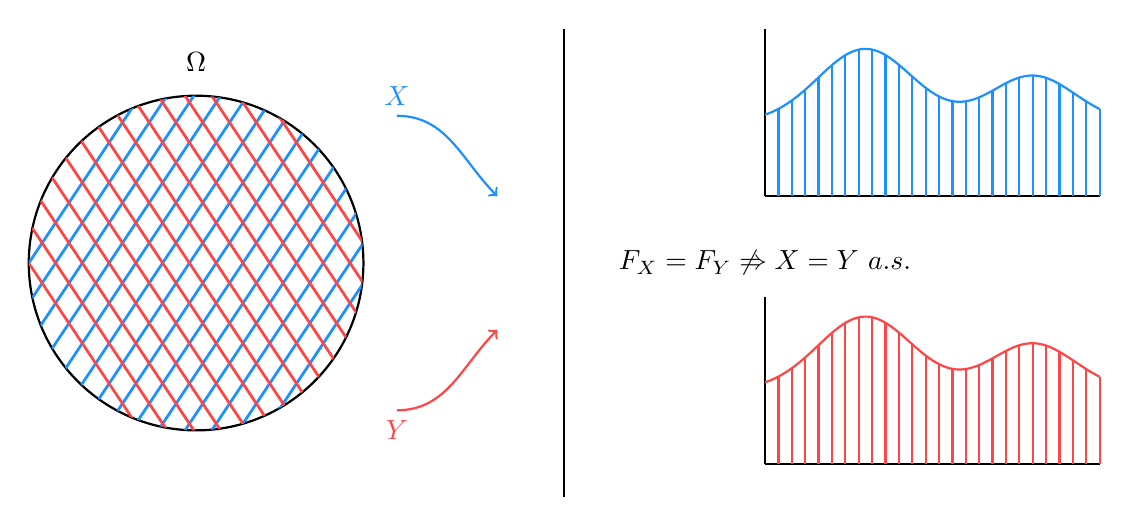
\begin{tikzpicture}[scale=0.85]
      % Define colors
      \definecolor{xcolor}{RGB}{30,144,255}  % Blue
      \definecolor{ycolor}{RGB}{255,70,70}   % Red
      
      % Load patterns library
      \usetikzlibrary{patterns}
      
      % Probability space (Omega)
      \begin{scope}
        \node at (-3.5,3) {$\Omega$};
        \draw[thick] (-3.5,0) circle (2.5);
        
        % Create custom patterns with proper colors and denser lines
        \begin{scope}
          % Blue lines pattern (X) - with reduced spacing between lines
          \clip (-3.5,0) circle (2.5);
          \foreach \i in {-8,-7.6,-7.2,...,5} {
            \draw[xcolor, line width=1.0pt] (\i,-3) -- (\i+4,3);
          }
        \end{scope}
        
        \begin{scope}
          % Red lines pattern (Y) - with reduced spacing between lines
          \clip (-3.5,0) circle (2.5);
          \foreach \i in {-8,-7.6,-7.2,...,2} {
            \draw[ycolor, line width=1.0pt] (\i+4,-3) -- (\i,3);
          }
        \end{scope}
      \end{scope}
      
      % X random variable label and arrow
      \node[xcolor] at (-0.5,2.5) {$X$};
      \draw[->, xcolor, thick, out=0, in=135] (-0.5,2.2) to (1,1);
      
      % Y random variable label and arrow
      \node[ycolor] at (-0.5,-2.5) {$Y$};
      \draw[->, ycolor, thick, out=0, in=225] (-0.5,-2.2) to (1,-1);
      
      % Vertical dividing line
      \draw[thick] (2,-3.5) -- (2,3.5);
      
      % Define distribution function once to ensure consistency
      \pgfmathdeclarefunction{distfunc}{1}{%
        \pgfmathparse{0.1+1.1*exp(-(#1-1.5)^2/1.0)+0.7*exp(-(#1-4)^2/0.8)}%
      }
      
      % X distribution (top right)
      \begin{scope}[shift={(5,2)}]
        \draw[thick] (0,-1) -- (5,-1);
        \draw[thick] (0,-1) -- (0,1.5);
        
        % Calculate curve points directly from the function to ensure alignment
        \draw[xcolor, thick] plot[smooth, domain=0:5, samples=50] 
          (\x, {distfunc(\x)});
        
        % Vertical lines for X distribution
        \foreach \i in {0.2,0.4,...,5} {
          \pgfmathsetmacro{\yval}{distfunc(\i)}
          \draw[xcolor, line width=0.8pt] (\i,-1) -- (\i,\yval);
        }
      \end{scope}
      
      % Relationship text
      \node at (5,0) {$F_X = F_Y \not\Rightarrow X=Y\ a.s.$};
      
      % Y distribution (bottom right)
      \begin{scope}[shift={(5,-2)}]
        \draw[thick] (0,-1) -- (5,-1);
        \draw[thick] (0,-1) -- (0,1.5);
        
        % Calculate curve points directly from the function to ensure alignment
        \draw[ycolor, thick] plot[smooth, domain=0:5, samples=50] 
          (\x, {distfunc(\x)});
        
        % Vertical lines for Y distribution
        \foreach \i in {0.2,0.4,...,5} {
          \pgfmathsetmacro{\yval}{distfunc(\i)}
          \draw[ycolor, line width=0.8pt] (\i,-1) -- (\i,\yval);
        }
      \end{scope}
    \end{tikzpicture}
    \caption{Two identical distributions may not model the same phenomenon.} 
    \label{fig:prob_in_dist}
  \end{figure}

  \begin{example}[C. in Distribution $\centernot\implies$ C. in Probability]
    Let $X_1, X_2, \ldots$ be such that $X_i = X$ for all $i$ where $X \sim \mathrm{Bernoulli}(1/2)$. This does not mean that the $X_i$'s are iid Bernoulli; they are all copies of the same $X$, i.e. forms a constant sequence. Let $Y = 1 - X$. Clearly, $X_n \xrightarrow{D} Y$ since the CDF of every $X_i$ is the same as that of $Y$, but $|X_n - Y| = 1$ for all $n$, so there is no convergence.  
  \end{example}

  \begin{example}[C. in Distribution $\centernot\implies$ C. in Probability]
    Let $X_1, X_2, \ldots \sim \mathcal{N}(0, 1)$ and $Y = -X$. Then, by symmetry of the standard Gaussian, both $X$ and $Y$ have the same CDF, but they are not the same random variable: their signs are opposite. 
  \end{example}

\subsection{Covariance and Correlation}

  The variance is a measure for one random variable $X$, which measures how much it deviates from its mean. Now, the covariance is defined for two random variables and captures how they jointly vary. 

  \begin{definition}[Covariance]
    The \textbf{covariance} of random variables $X$ and $Y$ is defined as 
    \begin{align*}
      \mathrm{Cov}[X, Y] & = \mathbb{E} \big[ (X - \mathbb{E}[X]) (Y - \mathbb{E}[X]) \big] \\
      & = \mathbb{E}[X Y] - \mathbb{E}[X] \, \mathbb{E}[Y]
    \end{align*}
    where the intermediate expectations are well-defined. $X$ and $Y$ are said to be \textbf{uncorrelated} if 
    \begin{equation}
      \mathrm{Cov}[X, Y] = 0
    \end{equation}
  \end{definition}

  The covariance is also easy to interpret. Given two random variables $X$ and $Y$, if whenever $X$ is greater than its expected value $\mathbb{E}[X]$, $Y$ also tends to be greater than $\mathbb{E}[Y]$, then the covariance will be some positive number. If they tend to be on opposite sides of their expected values, then the covariance will be negative. And the degree with which these RVs lie on which side of the expected value determines the magnitude of the covariance. 

  \begin{theorem}
    If $X$ and $Y$ are independent random variables, then they are uncorrelated, meaning that independence is a stronger condition. 
  \end{theorem}

  We show an example of why the converse is not true. Consider $X \sim \mathrm{Uniform}[-1, 1]$. We can show that $x$ and $Y = X^2$ are dependent but uncorrelated. It is clearly dependent, but its covariance is 
  \begin{align*}
    \mathrm{Cov}(X, Y) & = \mathbb{E}[X Y] - \mathbb{E}[X] \, \mathbb{E}[Y] \\
    & = \mathbb{E}[X^3] - \mathbb{E}[X] \, \mathbb{E}[X^2] \\
    & = \int_{-1}^1 x^3 \cdot 1 \,dx - 0 \cdot \mathbb{E}[X^2] = 0
  \end{align*}

  \begin{theorem}[Variance of Sums of Random Variables]
    If $X$ and $Y$ are two random variables, then 
    \begin{equation}
      \mathrm{Var}(X + Y) = \mathrm{Var}[X] + \mathrm{Var}(Y) + 2 \mathrm{Cov}(X, Y)
    \end{equation}
    and by induction, we can show that 
    \begin{equation}
      \mathrm{Var}\bigg( \sum_i X_i\bigg) = \sum_{i} \mathrm{Var}(X_i) + \sum_{i, j} \mathrm{Cov}(X_i, X_j)
    \end{equation}
  \end{theorem}
  \begin{proof}
    Simple computation. The LHS expands to 
    \begin{align*}
      \mathbb{E}[(X + Y)^2] - \mathbb{E}[X + Y]^2 & = \mathbb{E}[X^2 + 2XY + Y^2] - (\mathbb{E}[X] + \mathbb{E}[Y])^2 \\
      & = \mathbb{E}[X^2] + 2 \mathbb{E}[XY] + \mathbb{E}[Y^2] - \mathbb{E}[X]^2 - 2 \mathbb{E}[X] \mathbb{E}[Y] - \mathbb{E}[Y]^2 \\
      & = \big( \mathbb{E}[X^2] - \mathbb{E}[X]^2 \big) + \big( \mathbb{E}[Y^2] - \mathbb{E}[Y]^2 \big) + 2 \big( \mathbb{E}[XY] - \mathbb{E}[X] \mathbb{E}[Y] \big) \\
      & = \mathrm{Var}[X] + \mathrm{Var}(Y) + 2 \mathrm{Cov}(X, Y) 
    \end{align*}
  \end{proof}

  Therefore, if we have $n$ random variables $X_1, \ldots, X_n$, then we can compute their pairwise covariance $\mathrm{Cov}(X_i, X_j)$ and compute their \textbf{covariance matrix} $\boldsymbol{\Sigma}$, which is an $n \times n$ symmetric matrix with entries 
  \begin{equation}
    \boldsymbol{\Sigma}_{ij} = \mathrm{Cov}(X_i, X_j) \text{ for } i, j = 1, \ldots, n
  \end{equation}

  \begin{theorem}[Simple Bound on Covariance]
    If $X$ and $Y$ are two random variables with finite variance, then the magnitude of their covariance is bounded by the following inequality. 
    \begin{equation}
      |\Cov(X,Y)| \leq \sqrt{\Var(X) \, \Var(Y)} = \std(X) \, \std(Y)
    \end{equation}
  \end{theorem}

  Finally we define the correlation. 

  \begin{definition}[Correlation Coefficient]
    The \textbf{correlation coefficient} of random variables $X$ and $Y$ is defined 
    \begin{equation}
      \rho_{X, Y} = \mathrm{Corr}(X, Y) \coloneqq \frac{\mathrm{Cov}(X, Y)}{\sigma_X \sigma_Y} = \frac{\mathrm{Cov}(X, Y)}{\sqrt{\mathrm{Var}[X] \, \mathrm{Var}(Y)}}
    \end{equation}
  \end{definition}

  By definition, this implies that $-1 \leq \Corr(X, Y) \leq 1$. When $\Corr(X, Y) > 0$ (which also means that $\Cov(X, Y) > 0$), it is said that $X$ and $Y$ are \textit{positively correlated}, and when $\Corr(X, Y) < 0$ (which also means that $\Cov(X, Y) < 0$), it is said that they are \textit{negatively correlated}. 

  \begin{theorem}
    $\Corr(X,Y) = \pm 1$ indicates a linear relationship between $X$ and $Y$. 
    \begin{enumerate}
      \item Let $\Corr(X, Y) = 1$. Then, there exists a $m>0$ and $b \in \mathbb{R}$ such that $Y = m X + b$. 
      \item Let $\Corr(X, Y) = -1$. Then, there exists a $m<0$ and $b \in \mathbb{R}$ such tat $Y = m X + b$. 
    \end{enumerate}
    This implies that $\Corr(X, Y) = \pm 1$ indicates that the joint distribution of $(X, Y)$ is concentrated on a line in $\mathbb{R}^2$. 
  \end{theorem}

  In some sense the correlation is a scaled version of the covariance. It is scale-invariant, and it is always a number that lies between $-1$ and $1$, making it a nice way to represent the correlation between two variables without having to worry about scale. We can prove this. 

  \begin{theorem}[Cauchy-Schwartz]
    For any two random variables $X, Y$, we have $|\mathrm{Cov}(X, Y)| \leq \sigma_X \sigma_Y$, or in other words, 
    \begin{equation}
      -1 \leq \rho_{X, Y} \leq 1
    \end{equation}
    Furthermore, whenever $\rho_{X, Y} = 1$ or $-1$, there exists a deterministic relationship between $X$ and $Y$. 
    \begin{enumerate}
      \item If $\rho_{X, Y} = 1$, there exists a $a > 0$ s.t. 
      \begin{equation}
        Y - \mathbb{E}[Y] = a (X - \mathbb{E}[X])
      \end{equation}
      \item If $\rho_{X, Y} = -1$ there exists a $a < 0$ s.t. 
      \begin{equation}
        Y - \mathbb{E}[Y] = a (X - \mathbb{E}[X])
      \end{equation}
    \end{enumerate}
    This implies that $\Corr(X, Y) = \pm 1$ indicates that the joint distribution of $(X, Y)$ is concentrated on a line in $\mathbb{R}^2$. 
  \end{theorem}

  The fact that this is called the Cauchy-Schwartz inequality hints at the existence of inner products, norms, and vector spaces. That is, we can treat the random variables $X, Y$ as vectors in the functional space of real-valued maps over $\Omega$. In some sense, $\mathrm{Cov}(X, Y)$ sort-of plays the role of an inner product. 
  \begin{enumerate}
    \item It satisfies symmetricity: 
    \begin{equation}
      \mathrm{Cov}(X, Y) = \mathbb{E}[X Y] - \mathbb{E}[X] \, \mathbb{E}[Y] =  \mathbb{E}[Y X] - \mathbb{E}[Y] \, \mathbb{E}[X] = \mathrm{Cov}(Y, X)
    \end{equation}
    
    \item It satisfies binlinearity. It suffices to show only for first argument, since we have symmetricity. 
    \begin{align*}
      \mathrm{Cov}(aX + bY, Z) & = \mathbb{E}[(a X + b Y) Z] - \mathbb{E}[a X + b Y] \, \mathbb{E}[Z] \\
      & = a \mathbb{E}[X Z] + b \mathbb{E}[Y Z] - a \mathbb{E}[X] \mathbb{E}[Z] - b \mathbb{E}[Y] \, \mathbb{E}[Z] \\
      & = a \big( \mathbb{E}[X Z] - \mathbb{E}[X] \mathbb{E}[Z] \big) + a \big( \mathbb{E}[Y Z] - \mathbb{E}[Y] \, \mathbb{E}[Z] \big) \\
      & = a \, \mathrm{Cov}(X, Z) + b \, \mathrm{Cov}(Y, Z)
    \end{align*}

    \item We want the inner product of $X$ with itself to always be greater than $0$, with equality holding iff $X = 0$. Indeed, we have 
    \begin{equation}
      \mathrm{Cov}(X, X) = \mathrm{Var}[X] \geq 0
    \end{equation}
    but it is not necessarily true that $\mathrm{Var}[X] = 0 \implies X = 0$. We can say that $X$ is equal to a constant almost everywhere at best. We can solve this problem by looking at the functional subspace of $0$-mean random variables (which is a vector space due to linearity of expectation). So now all random variables $X$ that are $0$ almost everywhere have inner product $0$, so we must add an equivalence class on this subspace that says two $X, Y$ are equivalent if they agree almost everywhere. 
  \end{enumerate}

  The standard deviation $\sigma_X$ and $\sigma_Y$ act as norms on this quotient subspace of $0$-mean random variables. So the correlation coefficient $\rho_{X, Y}$ can be interpreted as the cosine of the angle between $X$ and $Y$. This now makes our desired space a Hilbert space, and our uncorrelated random variables are like orthogonal vectors. 

  \begin{definition}
    Let $L^2_\mathcal{F} (\Omega)$ be the function space consisting of equivalence classes of $0$-mean random variables $X: (\Omega, \mathcal{F}) \rightarrow \mathbb{R}$ that are almost surely equal. Then, 
    \begin{enumerate}
      \item we can define the inner product on this space as 
      \begin{equation}
        \langle X, Y \rangle \coloneqq \mathbb{E}[X Y] - \mathbb{E}[X] \mathbb{E}[Y] = \mathbb{E}[X Y] = \int_\Omega X Y \,d\mathbb{P}
      \end{equation}

      \item which induces the $L^2$-norm on this space defined 
      \begin{equation}
        ||X||_2 \coloneqq \mathrm{Var}(X) = \mathbb{E}[X^2] - \mathbb{E}[X]^2 = \mathbb{E}[X^2] = \int_\Omega X^2 \,d\mathbb{P}
      \end{equation}
    \end{enumerate}
    We set $L^2_\mathcal{F} (\Omega)$ to be a Banach space with bounded norm $\mathbb{E}[X^2] < \infty$. 
  \end{definition}

\subsection{Transforms}

  \subsubsection{Probability Generating Function (PGF)}

    The PGF is only defined for discrete random variable, and is analogous to the Z-transform in singal processing. 

    \begin{definition}[Probability Generating Function]
      Let $X$ be a discrete random variable taking values in $\mathbb{N}_0$. Then, the \textbf{probability generating function} of $X$ is defined 
      \begin{equation}
        G_X (z) \coloneqq \mathbb{E}[z^X] = \sum_{i=0}^\infty z^i \, \mathbb{P}(X = i)
      \end{equation}
      Now there is the problem of convergence, but we will not pay attention to this technicality for now and just consider the PGF as a tool. 
    \end{definition}

    \begin{example}[PGF of Poisson]
      The random variable $X \sim \mathrm{Poisson}(\lambda)$ has pmf $\mathbb{P}(X = i) = \frac{e^{-\lambda} \lambda^i}{i!}$ for $i \in \{0, 1, \ldots\}$. Then, 
      \begin{equation}
        G_X (z) = \mathbb{E}[z^X] = \sum_{i=0}^\infty z^i \, \frac{e^{-\lambda} \lambda^i}{i!} = \sum_{i=0}^\infty \frac{e^{-\lambda} (\lambda z)^i}{i!} = e^{\lambda(z - 1)}
      \end{equation}
    \end{example}

    \begin{example}[PGF of Geometric]
      For $X \sim \mathrm{Geometric}(p)$, its PGF is 
      \begin{equation}
        G_X (z) = \sum_{i=1}^\infty z^i \, (1 - p)^i p = \frac{p z}{1 - z(1 - p)}
      \end{equation}
    \end{example}

    \begin{lemma}[Properties of PGF]
      Given random variable $X$ and its PGF $G_X$, we have the following: 
      \begin{enumerate}
        \item Evaluate at $z = 1$: 
        \begin{equation}
          G_X (1) = \mathbb{E}[1^X] = \mathbb{E}[1] = 1
        \end{equation}
        \item Derivative at $z = 1$: 
        \begin{equation}
          \frac{d G_X (z)}{d z} \bigg|_{z = 1} = \mathbb{E}[X]
        \end{equation}
        \item $k$th derivative at $z = 1$: 
        \begin{equation}
          \frac{d^k G_X (z)}{d z^k} \bigg|_{z = 1} = \mathbb{E}[X (X-1) (X-2) \ldots (X-k +1)]
        \end{equation}
        \item Transformation: Given the sum $Z = X + Y$ (where $X, Y$ are independent), rather than computing its convolution, the PGF of $Z$ is simply the product of the PGFs of $X$ and $Y$: 
        \begin{equation}
          G_Z (z) = G_X (z) \, G_Y (z)
        \end{equation}
        For example, since a $\mathrm{Poisson}(\lambda)$ random variable has PGF of form $e^{\lambda (z - 1)}$, if we have two Poissons $X$ and $Y$ with parameters $\lambda, \mu$, then we can easily multiply their PGFs to get the PGF of $Z = X + Y$, which is $e^{(\lambda + \mu)(z - 1)}$, which is the PGF of a $\mathrm{Poisson}(\lambda + \mu)$ random variable. 
      \end{enumerate}
    \end{lemma}

  \subsubsection{Moment Generating Function (MGF)}

    \begin{definition}[Moment Generating Function (MGF)]
      The \textbf{moment generating function} associated with a random variable $X$ is a function $M_X: \mathbb{R} \longrightarrow [0, \infty]$ defined 
      \begin{equation}
        M_X (s) \coloneqq \mathbb{E}[e^{s X}]
      \end{equation}
      It is like an exponential moment. The region of convergence of $M_X$ is the set $D_X = \{s \mid M_X (s) < \infty\}$. 
      and we always have $M_X (0) = 1$, so $0 \in D_X$ always. 
    \end{definition}

    \begin{lemma}[Properties of MGF]
      Let $X$ be a random variable with MGF $M_X (s)$. 
      \begin{enumerate}
        \item $M_X (0) = 1$, so $0$ is always in the region of convergence. 
        \item If $Y = a X + b$, then 
        \begin{equation}
          M_Y (s) = e^{b s} M_X (a s)
        \end{equation}
        \item If $X$ and $Y$ are independent and $Z = X + Y$, then 
        \begin{equation}
          M_Z (s) = M_X (s) \, M_Y (s)
        \end{equation}
      \end{enumerate}
    \end{lemma}
    \begin{proof}
      Listed. 
      \begin{enumerate}
        \item $M_X (0) = \mathbb{E}[e^{0 X}] = \mathbb{E}[1] = 1$. 
        \item We have 
        \begin{align*}
          M_Y (s) & = \mathbb{E} [e^{s(a X + b)}] \\
          & = \mathbb{E}[ e^{a s X } e^{b s}] \\
          & = \mathbb{E}[e^{(as) X}] \, \mathbb{E}[e^{b s}] \\
          & = e^{b s} M_X (a s)
        \end{align*}
        where the penultimate step was due to independence of constant RV with any other RVs. 
        \item We can see 
        \begin{equation}
          M_Z (s) = \mathbb{E}[ e^{s (X + Y)}] = \mathbb{E}[e^{s X} \, e^{s Y}] = \mathbb{E}[e^{s X}] \, \mathbb{E}[e^{s Y}] = M_X (s) \, M_Y (s)
        \end{equation}
        since $X, Y$ independent means that any function of $X$ and $Y$ are independent. 
      \end{enumerate}
    \end{proof}

    \begin{theorem}[Inversion Theorem]
      Suppose $M_X (s)$ is finite for all $s \in [-\epsilon, \epsilon]$ for some $\epsilon > 0$. Then, $M_X$ uniquely determines the CDF of $X$. This implies that if $X$ and $Y$ are random variables such that $M_X (s) = M_Y (s)$ for all $s \in [-\epsilon, \epsilon]$ for some $\epsilon > 0$, then $X$ and $Y$ have the same CDF. 
    \end{theorem}

    This theorem is useful for comparing random variables with the MGFs, but a limitation is that it is not always clear that the MGF is defined beyond $0$. Now, we explain why this is called a moment generating function. 

    \begin{theorem}[Moment Generating Property]
      Suppose $M_X (s) < \infty$ for $s \in [-\epsilon, \epsilon]$ with $\epsilon > 0$. Then, the derivatives at $s = 0$ generate the moments of $X$: 
      \begin{equation}
        \frac{d^m M_X (s)}{d s^m} \bigg|_{s = 0} = \mathbb{E}[X^m]
      \end{equation}
    \end{theorem}
    \begin{proof}
      A hand-wavy proof is that we can take the derivative and put it "in" the expectation. 
      \begin{equation}
        \frac{d}{ds} \mathbb{E}[e^{s X}] = \mathbb{E} \big[ \frac{d}{ds} e^{s X} \big] = \mathbb{E}[X e^{s X}]
      \end{equation}
      which evaluates to $\mathbb{E}[X]$ when $s = 0$. Differentiating $m$ times just gets $\mathbb{E}[X^m e^{s X}]$. However, this should be questioned, since the expectation is an integral and we are putting the derivative inside the integral. 
    \end{proof}

    \begin{example}[Exponential RV]
      The PDF of $X \sim \mathrm{Exponential}(\mu)$ is $f_X (x) = \mu e^{-\mu x}$ for $x \geq 0$. The MGF is 
      \begin{equation}
        M_X (s) \coloneqq \int_0^\infty \mu e^{-\mu x} e^{s x} \, dx = \begin{cases} 
        \frac{\mu}{\mu - s} & \text{ for } s < \mu \\
        \infty & \text{ for } s \geq \mu 
      \end{cases}
      \end{equation}
    \end{example}

    \begin{example}[Gaussian RV]
      The PDF of a standard Gaussian $X$ is $f_X (x) = \frac{1}{\sqrt{2\pi}} e^{-x^2 / 2}$ for $x \in \mathbb{R}$, and the MGF is 
      \begin{equation}
        M_X (s) = \int_{-\infty}^\infty \frac{1}{\sqrt{2 \pi}} e^{- x^2 / 2} e^{s x} \,dx = e^{s^2 / 2} \int_{-\infty}^\infty \frac{1}{\sqrt{2\pi}} e^{-\frac{(x - s)^2}{2}}\,dx = e^{s^2 / 2}
      \end{equation}
      which is valid for all $s \in \mathbb{R}$. 
    \end{example}

    \begin{example}[Cauchy RV]
      If we have $f_X (x) = \frac{1}{\pi} \frac{1}{1 + x^2}$ for $x \in \mathbb{R}$, the MGF is 
      \begin{equation}
        M_X (s) = \int_{-\infty}^\infty \frac{e^{s x}}{\pi (1 + x^2)} \,dx = \begin{cases} 1 & \text{ if } s = 0 \\
        \infty & \text{ if } s > 0 \\ 
        \infty & \text{ if } s < 0 \end{cases}
      \end{equation}
      So the region of convergence is just $\{0\}$. It is infinity everywhere else since the exponential function grows exponentially as $x \rightarrow \pm \infty$. 
    \end{example}

    \begin{example}
      Given $X_1 \sim \mathrm{Exponential}(\lambda_1)$ and $X_2 \sim \mathrm{Exponential}(\lambda_2)$ are independent, the MGF of $Z = X_1 + X_2$ is 
      \begin{equation}
        M_Z (s) = M_X (s) \, M_Y (s) = \frac{\lambda_1 \lambda_2}{(\lambda_1 - s)(\lambda_2 - s)} \text{ for } s < \min\{\lambda_1, \lambda_2\}
      \end{equation}
      and we can perform our inverse transform on it. 
    \end{example}

  \subsubsection{Characteristic Function}

    We can see that the MGF has its limitations: for some random variables (like the Cauchy), its MGF was not defined at all beyond $\{0\}$. On the contrary, the characteristic function is always defined everywhere and is finite everywhere (in fact, is bounded by $1$, shown below). Also, it is a bit easier to invert (similar to how the Fourier transform is a bit easier to invert than the Laplace). 

    \begin{definition}[Characteristic Function]
      Given a random variable $X: \Omega \longrightarrow \mathbb{R}$, the \textbf{characteristic function} is defined to be 
      \begin{align*}
        \varphi_X (t) & = \mathbb{E}[ e^{i t X} ] \\
        & = \mathbb{E}[\cos{(t X)}] + i \mathbb{E}[ \sin{(t X)}]
      \end{align*}
    \end{definition}

    If $X$ admits a PDF, then the characteristic function is its Fourier transform with a small sign reversal. 
    \begin{equation}
      \varphi_X (t) = \int_\mathbb{R} e^{i t x} f_X (x)\,dx
    \end{equation}

    \begin{theorem}[Properties of CF]
      Let $X$ be a random variable with CF $\varphi_X (t)$. 
      \begin{enumerate}
        \item $\varphi_X (0) = 1$  and $|\varphi_X (t)| \leq 1$ for all $t \in \mathbb{R}$. 
        \item If $Y = a X + b$, then 
        \begin{equation}
          \varphi_Y (t) = e^{i b t} \varphi_X (a t)
        \end{equation}
        \item If $X$ and $Y$ are independent random variables and $Z = X + Y$, then 
        \begin{equation}
          \varphi_Z (t) = \varphi_X (t) \, \varphi_Y (t)
        \end{equation}
        \item $\varphi_X (t)$ is uniformly continuous on $\mathbb{R}$, i.e. for all $t \in \mathbb{R}$, there exists a $\phi(h) \downarrow 0$ as $h \downarrow 0$ such that 
        \begin{equation}
          |\varphi_X (t + h) - \varphi_X (t)| \leq \phi(h)
        \end{equation}
        \item $\varphi_X$ is a nonnegative-definite kernel, i.e. for any $n$ reals $t_1, \ldots, t_n$ and $n$ complex numbers $z_1, \ldots z_n$, we have 
        \begin{equation}
          \sum_{i, j} z_i \varphi_X (t_i - t_j) \, \bar{z}_j \geq 0
        \end{equation}
      \end{enumerate}
    \end{theorem}
    \begin{proof}
      Listed. 
      \begin{enumerate}
        \item We just set $\varphi_X (0) = \mathbb{E}[e^{i 0 X}] = \mathbb{E}[1] = 1$, and for continuous random variables, we can bound 
        \begin{align*}
          \big| \varphi_X (t) \big| & = \bigg| \int_{-\infty}^\infty e^{i t x} f_X (x) \,dx  \bigg| \\
          & \leq \int_{-\infty}^\infty \big| e^{i t x} f_X (x) \big| \,dx \\
          & \leq \int_{-\infty}^\infty \big| e^{i t x} \big| \cdot \big|f_X (x) \big| \,dx \\
          & = \int_{-\infty}^\infty f_X (x) \,dx = 1 
        \end{align*}
        
        \item We have 
        \begin{equation}
          \varphi_Y (t) = \mathbb{E}[ e^{i t (a X + b)}] = \mathbb{E}[ e^{i a t X} \, e^{i b t}] = \mathbb{E}[ e^{i (at) X}] \, \mathbb{E}[e^{i b t}] = e^{i b t} \varphi_X (a t)
        \end{equation}
        
        \item We have 
        \begin{equation}
          \varphi_Z (t) = \mathbb{E}[ e^{i t (X + Y)}] = \mathbb{E}[ e^{i t X} \, e^{i t Y}] = \mathbb{E}[e^{i t X}] \, \mathbb{E}[e^{i t Y}] = \varphi_X (t) \, \varphi_Y (t)
        \end{equation}
        
        \item We have 
        \begin{align*}
          | \varphi_X (t + h) - \varphi_X (t)| & = | \mathbb{E} [ e^{i tX} (e^{i h X} - 1)] | \\ 
          & \leq \mathbb{E}[ | e^{i tX} (e^{i h X} - 1)|] \\
          & \leq \mathbb{E}[ |e^{i h X} - 1|] \ldots
        \end{align*}
      \end{enumerate}
    \end{proof}

    Now this next theorem states the uniqueness of each characteristic function. It is a highly nontrivial result. 

    \begin{theorem}[Inversion Theorem]
      If two random variables have the same characteristic function, then their CDFs are the same. Further, if $X$ is a continuous random variable, then the PDF can be recovered from the characteristic function as follows: 
      \begin{equation}
        f_X (x) = \lim_{T \rightarrow \infty} \frac{1}{2 \pi} \int_{-T}^T e^{- i t x} \varphi_X (t) \,dt
      \end{equation}
      for every $x$ where $f_X (x)$ is continuous. 
    \end{theorem}

    Just like how we can recover moments from the MGF, we can always recover the moments from the characteristic function, with the added advantage that the CF will always exist. 

    \begin{theorem}[Moment Generating Property]
      Let $X$ be a random variable and $\varphi_X (t)$ its CF. 
      \begin{enumerate}
        \item If $\varphi_X^{(k)} (t)$ ( the $k$th derivative) exists at $t = 0$, then 
        \begin{align*}
          \mathbb{E}[|X^k|] < \infty & \text{ for } k \text{ even} \\
          \mathbb{E}[|X^{k-1}|] < \infty & \text{ for } k \text{ odd}
        \end{align*}
        
        \item If $\mathbb{E}[|X^k|] < \infty$, then 
        \begin{equation}
          \varphi_X^{(k)} (0) = i^k \mathbb{E}[X^k]
        \end{equation}
        
        \item Further, given that the moments are finite, we can expand the CF by moments of $X$ as 
        \begin{equation}
          \varphi_X (t) = \sum_{j=0}^k \frac{\mathbb{E}[X^j]}{j!} (i t)^j + o(t^k)
        \end{equation}
      \end{enumerate}
    \end{theorem}

    \begin{example}[Bernoulli]
      Given $X \sim \mathrm{Bernoulli}(p)$, we have 
      \begin{align*}
        \mathbb{E}[ e^{i t X}] & = \sum_{x \in \{0, 1\}} e^{i t x} \cdot \mathbb{P}(X = x) \\
        & = e^{i t 0} (1 - p) + e^{i t} p \\
        & = 1 - p + p e^{i t}
      \end{align*}
    \end{example}

    \begin{example}[Exponential]
      Given $X \in \mathrm{Exponential}(\lambda)$, we have 
      \begin{align*}
        \mathbb{E}[e^{i t X}] & = \int_0^\infty e^{i t x} \lambda e^{-\lambda x} \,dx \\
        & = \int_0^\infty \lambda \, e^{-(\lambda - i t) x} \,dx \\
        & = \frac{\lambda}{\lambda - it} \text{ for all } t \in \mathbb{R}
      \end{align*}
      where the complex integral requires some complex analysis. 
    \end{example}

\subsection{Exercises}

  \begin{exercise}[Durrett 1.3.1]
    Show that if $\mathcal{A}$ generates $\mathcal{S}$, then $X^{-1}(\mathcal{A}) \equiv \{\{X \in A\} : A \in \mathcal{A}\}$ generates $\sigma(X) = \{\{X \in B\} : B \in \mathcal{S}\}$.
  \end{exercise}
  \begin{solution}

  \end{solution}

  \begin{exercise}[Durrett 1.3.2]
    Prove Theorem 1.3.6 when $n = 2$ by checking $\{X_1 + X_2 < x\} \in \mathcal{F}$.
  \end{exercise}
  \begin{solution}

  \end{solution}

  \begin{exercise}[Durrett 1.3.3]
    Show that if $f$ is continuous and $X_n \to X$ almost surely then $f(X_n) \to f(X)$ almost surely.
  \end{exercise}
  \begin{solution}

  \end{solution}

  \begin{exercise}[Durrett 1.3.4]
    \begin{enumerate}
      \item Show that a continuous function from $\mathbf{R}^d \to \mathbf{R}$ is a measurable map from $(\mathbf{R}^d, \mathcal{R}^d)$ to $(\mathbf{R}, \mathcal{R})$.
      \item Show that $\mathcal{R}^d$ is the smallest $\sigma$-field that makes all the continuous functions measurable.
    \end{enumerate}
  \end{exercise}
  \begin{solution}

  \end{solution}

  \begin{exercise}[Durrett 1.3.5]
    A function $f$ is said to be \textbf{lower semicontinuous} or l.s.c. if
    \begin{equation*}
      \liminf_{y \to x} f(y) \geq f(x)
    \end{equation*}
    and \textbf{upper semicontinuous} (u.s.c.) if $-f$ is l.s.c. Show that $f$ is l.s.c. if and only if $\{x : f(x) \leq a\}$ is closed for each $a \in \mathbf{R}$ and conclude that semicontinuous functions are measurable.
  \end{exercise}
  \begin{solution}

  \end{solution}

  \begin{exercise}[Durrett 1.3.6]
    Let $f : \mathbf{R}^d \to \mathbf{R}$ be an arbitrary function and let $f^{\delta}(x) = \sup\{f(y) : |y - x| < \delta\}$ and $f_{\delta}(x) = \inf\{f(y) : |y - x| < \delta\}$ where $|z| = (z_1^2 + \dots + z_d^2)^{1/2}$. Show that $f^{\delta}$ is l.s.c. and $f_{\delta}$ is u.s.c. Let $f^0 = \lim_{\delta \downarrow 0} f^{\delta}$, $f_0 = \lim_{\delta \downarrow 0} f_{\delta}$, and conclude that the set of points at which $f$ is discontinuous $= \{f^0 \neq f_0\}$ is measurable.
  \end{exercise}
  \begin{solution}

  \end{solution}

  \begin{exercise}[Durrett 1.3.7]
    A function $\varphi : \Omega \to \mathbf{R}$ is said to be \textbf{simple} if
    \begin{equation*}
      \varphi(\omega) = \sum_{m=1}^{n} c_m 1_{A_m}(\omega)
    \end{equation*}
    where the $c_m$ are real numbers and $A_m \in \mathcal{F}$. Show that the class of $\mathcal{F}$ measurable functions is the smallest class containing the simple functions and closed under pointwise limits.
  \end{exercise}
  \begin{solution}

  \end{solution}

  \begin{exercise}[Durrett 1.3.8]
    Use the previous exercise to conclude that $Y$ is measurable with respect to $\sigma(X)$ if and only if $Y = f(X)$ where $f : \mathbf{R} \to \mathbf{R}$ is measurable.
  \end{exercise}
  \begin{solution}

  \end{solution}

  \begin{exercise}[Durrett 1.3.9]
    To get a constructive proof of the last result, note that $\{\omega : m 2^{-n} \leq Y < (m + 1)2^{-n}\} = \{X \in B_{m,n}\}$ for some $B_{m,n} \in \mathcal{R}$ and set $f_n(x) = m 2^{-n}$ for $x \in B_{m,n}$ and show that as $n \to \infty$ $f_n(x) \to f(x)$ and $Y = f(X)$.
  \end{exercise}
  \begin{solution}

  \end{solution}

  \begin{exercise}[Durrett 1.4.1]
    Show that if $f \geq 0$ and $\int f \, d\mu = 0$ then $f = 0$ a.e.
  \end{exercise}
  \begin{solution}

  \end{solution}

  \begin{exercise}[Durrett 1.4.2]
    Let $f \geq 0$ and $E_{n,m} = \{x : m/2^n \leq f(x) < (m + 1)/2^n\}$. As $n \uparrow \infty$,
    \begin{equation*}
      \sum_{m=1}^{\infty} \frac{m}{2^n} \mu(E_{n,m}) \uparrow \int f \, d\mu
    \end{equation*}
  \end{exercise}
  \begin{solution}

  \end{solution}

  \begin{exercise}[Durrett 1.4.3]
    Let $g$ be an integrable function on $\mathbf{R}$ and $\epsilon > 0$.
    \begin{enumerate}
      \item Use the definition of the integral to conclude there is a simple function $\varphi = \sum_{k} b_k 1_{A_k}$ with $\int |g - \varphi| \, dx < \epsilon$.
      \item Use Exercise A.2.1 to approximate the $A_k$ by finite unions of intervals to get a \textbf{step function}
      \begin{equation*}
        q = \sum_{j=1}^{k} c_j 1_{(a_{j-1}, a_j)}
      \end{equation*}
      with $a_0 < a_1 < \dots < a_k$, so that $\int |\varphi - q| < \epsilon$.
      \item Round the corners of $q$ to get a continuous function $r$ so that $\int |q - r| \, dx < \epsilon$.
    \end{enumerate}
  \end{exercise}
  \begin{solution}

  \end{solution}

  \begin{exercise}[Durrett 1.4.4]
    Prove the \textbf{Riemann-Lebesgue lemma}. If $g$ is integrable then
    \begin{equation*}
      \lim_{n \to \infty} \int g(x) \cos nx \, dx = 0
    \end{equation*}
    Hint: If $g$ is a step function, this is easy. Now use the previous exercise.
  \end{exercise}
  \begin{solution}

  \end{solution}

  \begin{exercise}[Durrett 1.5.1]
    Let $\|f\|_{\infty} = \inf\{M : \mu(\{x : |f(x)| > M\}) = 0\}$. Prove that
    \begin{equation*}
      \int |fg| \, d\mu \leq \|f\|_1 \|g\|_{\infty}
    \end{equation*}
  \end{exercise}
  \begin{solution}

  \end{solution}

  \begin{exercise}[Durrett 1.5.2]
    Show that if $\mu$ is a probability measure then
    \begin{equation*}
      \|f\|_{\infty} = \lim_{p \to \infty} \|f\|_p
    \end{equation*}
  \end{exercise}
  \begin{solution}

  \end{solution}

  \begin{exercise}[Durrett 1.5.3]
    \textbf{Minkowski's inequality.}
    \begin{enumerate}
      \item Suppose $p \in (1, \infty)$. The inequality $|f + g|^p \leq 2^p(|f|^p + |g|^p)$ shows that if $\|f\|_p$ and $\|g\|_p$ are $< \infty$ then $\|f + g\|_p < \infty$. Apply H\"{o}lder's inequality to $|f| |f + g|^{p-1}$ and $|g| |f + g|^{p-1}$ to show $\|f + g\|_p \leq \|f\|_p + \|g\|_p$.
      \item Show that the last result remains true when $p = 1$ or $p = \infty$.
    \end{enumerate}
  \end{exercise}
  \begin{solution}

  \end{solution}

  \begin{exercise}[Durrett 1.5.4]
    If $f$ is integrable and $E_m$ are disjoint sets with union $E$ then
    \begin{equation*}
      \sum_{m=0}^{\infty} \int_{E_m} f \, d\mu = \int_E f \, d\mu
    \end{equation*}
    So if $f \geq 0$, then $\nu(E) = \int_E f \, d\mu$ defines a measure.
  \end{exercise}
  \begin{solution}

  \end{solution}

  \begin{exercise}[Durrett 1.5.5]
    If $g_n \uparrow g$ and $\int g_1^- \, d\mu < \infty$ then $\int g_n \, d\mu \uparrow \int g \, d\mu$.
  \end{exercise}
  \begin{solution}

  \end{solution}

  \begin{exercise}[Durrett 1.5.6]
    If $g_m \geq 0$ then $\int \sum_{m=0}^{\infty} g_m \, d\mu = \sum_{m=0}^{\infty} \int g_m \, d\mu$.
  \end{exercise}
  \begin{solution}

  \end{solution}

  \begin{exercise}[Durrett 1.5.7]
    Let $f \geq 0$.
    \begin{enumerate}
      \item Show that $\int f \wedge n \, d\mu \uparrow \int f \, d\mu$ as $n \to \infty$.
      \item Use (i) to conclude that if $g$ is integrable and $\epsilon > 0$ then we can pick $\delta > 0$ so that $\mu(A) < \delta$ implies $\int_A |g| \, d\mu < \epsilon$.
    \end{enumerate}
  \end{exercise}
  \begin{solution}

  \end{solution}

  \begin{exercise}[Durrett 1.5.8]
    Show that if $f$ is integrable on $[a, b]$, $g(x) = \int_{[a, x]} f(y) \, dy$ is continuous on $(a, b)$.
  \end{exercise}
  \begin{solution}

  \end{solution}

  \begin{exercise}[Durrett 1.5.9]
    Show that if $f$ has $\|f\|_p = (\int |f|^p \, d\mu)^{1/p} < \infty$, then there are simple functions $\varphi_n$ so that $\|\varphi_n - f\|_p \to 0$.
  \end{exercise}
  \begin{solution}

  \end{solution}

  \begin{exercise}[Durrett 1.5.10]
    Show that if $\sum_n \int |f_n| \, d\mu < \infty$ then $\sum_n \int f_n \, d\mu = \int \sum_n f_n \, d\mu$.
  \end{exercise}
  \begin{solution}

  \end{solution}

  \begin{exercise}[Durrett 1.6.1]
    Suppose $\varphi$ is strictly convex, i.e., $>$ holds for $\lambda \in (0, 1)$. Show that, under the assumptions of Theorem 1.6.2, $\varphi(EX) = E\varphi(X)$ implies $X = EX$ a.s.
  \end{exercise}
  \begin{solution}

  \end{solution}

  \begin{exercise}[Durrett 1.6.2]
    Suppose $\varphi : \mathbf{R}^n \to \mathbf{R}$ is convex. Imitate the proof of Theorem 1.5.1 to show
    \begin{equation*}
      E\varphi(X_1, \dots, X_n) \geq \varphi(EX_1, \dots, EX_n)
    \end{equation*}
    provided $E|\varphi(X_1, \dots, X_n)| < \infty$ and $E|X_i| < \infty$ for all $i$.
  \end{exercise}
  \begin{solution}

  \end{solution}

  \begin{exercise}[Durrett 1.6.3]
    \textbf{Chebyshev's inequality is and is not sharp.}
    \begin{enumerate}
      \item Show that Theorem 1.6.4 is sharp by showing that if $0 < b \leq a$ are fixed there is an $X$ with $EX^2 = b^2$ for which $P(|X| \geq a) = b^2/a^2$.
      \item Show that Theorem 1.6.4 is not sharp by showing that if $X$ has $0 < EX^2 < \infty$ then
      \begin{equation*}
        \lim_{a \to \infty} a^2 P(|X| \geq a) / EX^2 = 0
      \end{equation*}
    \end{enumerate}
  \end{exercise}
  \begin{solution}

  \end{solution}

  \begin{exercise}[Durrett 1.6.4]
    \textbf{One-sided Chebyshev bound.}
    \begin{enumerate}
      \item Let $a > b > 0$, $0 < p < 1$, and let $X$ have $P(X = a) = p$ and $P(X = -b) = 1 - p$. Apply Theorem 1.6.4 to $\varphi(x) = (x + b)^2$ and conclude that if $Y$ is any random variable with $EY = EX$ and $\text{var}(Y) = \text{var}(X)$, then $P(Y \geq a) \leq p$ and equality holds when $Y = X$.
      \item Suppose $EY = 0$, $\text{var}(Y) = \sigma^2$, and $a > 0$. Show that $P(Y \geq a) \leq \sigma^2 / (a^2 + \sigma^2)$, and there is a $Y$ for which equality holds.
    \end{enumerate}
  \end{exercise}
  \begin{solution}

  \end{solution}

  \begin{exercise}[Durrett 1.6.5]
    \textbf{Two nonexistent lower bounds.} Show that:
    \begin{enumerate}
      \item if $\epsilon > 0$, $\inf \{P(|X| > \epsilon) : EX = 0, \text{var}(X) = 1\} = 0$.
      \item if $y \geq 1, \sigma^2 \in (0, \infty)$, $\inf \{P(|X| > y) : EX = 1, \text{var}(X) = \sigma^2\} = 0$.
    \end{enumerate}
  \end{exercise}
  \begin{solution}

  \end{solution}

  \begin{exercise}[Durrett 1.6.6]
    \textbf{A useful lower bound.} Let $Y \geq 0$ with $EY^2 < \infty$. Apply the Cauchy-Schwarz inequality to $Y 1_{\{Y > 0\}}$ and conclude
    \begin{equation*}
      P(Y > 0) \geq (EY)^2 / EY^2
    \end{equation*}
  \end{exercise}
  \begin{solution}

  \end{solution}

  \begin{exercise}[Durrett 1.6.7]
    Let $\Omega = (0, 1)$ equipped with the Borel sets and Lebesgue measure. Let $\alpha \in (1, 2)$ and $X_n = n^{\alpha} 1_{(1/(n+1), 1/n)} \to 0$ a.s. Show that Theorem 1.6.8 can be applied with $h(x) = x$ and $g(x) = |x|^{2/\alpha}$, but the $X_n$ are not dominated by an integrable function.
  \end{exercise}
  \begin{solution}

  \end{solution}

  \begin{exercise}[Durrett 1.6.8]
    Suppose that the probability measure $\mu$ has $\mu(A) = \int_A f(x) \, dx$ for all $A \in \mathcal{R}$. Use the proof technique of Theorem 1.6.9 to show that for any $g$ with $g \geq 0$ or $\int |g(x)| \mu(dx) < \infty$ we have
    \begin{equation*}
      \int g(x) \mu(dx) = \int g(x) f(x) \, dx
    \end{equation*}
  \end{exercise}
  \begin{solution}

  \end{solution}

  \begin{exercise}[Durrett 1.6.9]
    \textbf{Inclusion-exclusion formula.} Let $A_1, A_2, \dots, A_n$ be events and $A = \cup_{i=1}^{n} A_i$. Prove that $1_A = 1 - \prod_{i=1}^n (1 - 1_{A_i})$. Expand out the right hand side, then take expected value to conclude
    \begin{align*}
      P(\cup_{i=1}^n A_i) &= \sum_{i=1}^n P(A_i) - \sum_{i<j} P(A_i \cap A_j) \\
      &\quad + \sum_{i<j<k} P(A_i \cap A_j \cap A_k) - \dots + (-1)^{n-1} P(\cap_{i=1}^n A_i)
    \end{align*}
  \end{exercise}
  \begin{solution}

  \end{solution}

  \begin{exercise}[Durrett 1.6.10]
    \textbf{Bonferroni inequalities.} Let $A_1, A_2, \dots, A_n$ be events and $A = \cup_{i=1}^n A_i$. Show that $1_A \leq \sum_{i=1}^n 1_{A_i}$, etc. and then take expected values to conclude
    \begin{align*}
      P(\cup_{i=1}^n A_i) &\leq \sum_{i=1}^n P(A_i) \\
      P(\cup_{i=1}^n A_i) &\geq \sum_{i=1}^n P(A_i) - \sum_{i<j} P(A_i \cap A_j) \\
      P(\cup_{i=1}^n A_i) &\leq \sum_{i=1}^n P(A_i) - \sum_{i<j} P(A_i \cap A_j) + \sum_{i<j<k} P(A_i \cap A_j \cap A_k)
    \end{align*}
    In general, if we stop the inclusion exclusion formula after an even (odd) number of sums, we get a lower (upper) bound.
  \end{exercise}
  \begin{solution}

  \end{solution}

  \begin{exercise}[Durrett 1.6.11]
    If $E|X|^k < \infty$ then for $0 < j < k$, $E|X|^j < \infty$, and furthermore
    \begin{equation*}
      E|X|^j \leq (E|X|^k)^{j/k}
    \end{equation*}
  \end{exercise}
  \begin{solution}

  \end{solution}

  \begin{exercise}[Durrett 1.6.12]
    Apply Jensen's inequality with $\varphi(x) = e^x$ and $P(X = \log y_m) = p(m)$ to conclude that if $\sum_{m=1}^n p(m) = 1$ and $p(m), y_m > 0$ then
    \begin{equation*}
      \sum_{m=1}^n p(m) y_m \geq \prod_{m=1}^n y_m^{p(m)}
    \end{equation*}
    When $p(m) = 1/n$, this says the arithmetic mean exceeds the geometric mean.
  \end{exercise}
  \begin{solution}

  \end{solution}

  \begin{exercise}[Durrett 1.6.13]
    If $EX_1^- < \infty$ and $X_n \uparrow X$ then $EX_n \uparrow EX$.
  \end{exercise}
  \begin{solution}

  \end{solution}

  \begin{exercise}[Durrett 1.6.14]
    Let $X \geq 0$ but do NOT assume $E(1/X) < \infty$. Show
    \begin{equation*}
      \lim_{y \to \infty} y E(1/X; X > y) = 0, \quad \lim_{y \downarrow 0} y E(1/X; X > y) = 0.
    \end{equation*}
  \end{exercise}
  \begin{solution}

  \end{solution}

  \begin{exercise}[Durrett 1.6.15]
    If $X_n \geq 0$ then $E(\sum_{n=0}^{\infty} X_n) = \sum_{n=0}^{\infty} EX_n$.
  \end{exercise}
  \begin{solution}

  \end{solution}

  \begin{exercise}[Durrett 1.6.16]
    If $X$ is integrable and $A_n$ are disjoint sets with union $A$ then
    \begin{equation*}
      \sum_{n=0}^{\infty} E(X; A_n) = E(X; A)
    \end{equation*}
    i.e., the sum converges absolutely and has the value on the right.
  \end{exercise}
  \begin{solution}

  \end{solution}

  \begin{exercise}[Durrett 1.7.1]
    If $\int_X \int_Y |f(x, y)| \mu_2(dy) \mu_1(dx) < \infty$ then
    \begin{equation*}
      \int_X \int_Y f(x, y) \mu_2(dy) \mu_1(dx) = \int_{X \times Y} f \, d(\mu_1 \times \mu_2) = \int_Y \int_X f(x, y) \mu_1(dx) \mu_2(dy)
    \end{equation*}
    \textbf{Corollary.} Let $X = \{1, 2, \dots \}$, $\mathcal{A} =$ all subsets of $X$, and $\mu_1 =$ counting measure. If $\sum_n \int |f_n| d\mu < \infty$ then $\sum_n \int f_n d\mu = \int \sum_n f_n d\mu$.
  \end{exercise}
  \begin{solution}

  \end{solution}

  \begin{exercise}[Durrett 1.7.2]
    Let $g \geq 0$ be a measurable function on $(X, \mathcal{A}, \mu)$. Use Theorem 1.7.2 to conclude that
    \begin{equation*}
      \int_X g \, d\mu = (\mu \times \lambda)(\{(x, y) : 0 \leq y < g(x)\}) = \int_0^{\infty} \mu(\{x : g(x) > y\}) \, dy
    \end{equation*}
  \end{exercise}
  \begin{solution}

  \end{solution}

  \begin{exercise}[Durrett 1.7.3]
    Let $F, G$ be Stieltjes measure functions and let $\mu, \nu$ be the corresponding measures on $(\mathbf{R}, \mathcal{R})$. Show that
    \begin{enumerate}
      \item $\int_{(a, b]} \{F(y) - F(a)\} dG(y) = (\mu \times \nu)(\{(x, y) : a < x \leq y \leq b\})$
      \item $\int_{(a, b]} F(y) dG(y) + \int_{(a, b]} G(y) dF(y) = F(b)G(b) - F(a)G(a) + \sum_{x \in (a, b]} \mu(\{x\})\nu(\{x\})$
      \item If $F = G$ is continuous then $\int_{(a, b]} 2F(y) dF(y) = F^2(b) - F^2(a)$.
    \end{enumerate}
    To see the second term in (ii) is needed, let $F(x) = G(x) = 1_{[0, \infty)}(x)$ and $a < 0 < b$.
  \end{exercise}
  \begin{solution}

  \end{solution}

  \begin{exercise}[Durrett 1.7.4]
    Let $\mu$ be a finite measure on $\mathbf{R}$ and $F(x) = \mu((-\infty, x])$. Show that
    \begin{equation*}
      \int (F(x + c) - F(x)) \, dx = c \mu(\mathbf{R})
    \end{equation*}
  \end{exercise}
  \begin{solution}

  \end{solution}

  \begin{exercise}[Durrett 1.7.5]
    Show that $e^{-xy} \sin x$ is integrable in the strip $0 < x < a$, $0 < y$. Perform the double integral in the two orders to get:
    \begin{equation*}
      \int_0^a \frac{\sin x}{x} dx = \arctan(a) - (\cos a) \int_0^{\infty} \frac{e^{-ay}}{1 + y^2} dy - (\sin a) \int_0^{\infty} \frac{ye^{-ay}}{1 + y^2} dy
    \end{equation*}
    and replace $1 + y^2$ by 1 to conclude $|\int_0^a (\sin x)/x \, dx - \arctan(a)| \leq 2/a$ for $a \geq 1$.
  \end{exercise}
  \begin{solution}

  \end{solution}
